\documentclass{article}

% Remember to also load the algostyle.sty file into your project.
\usepackage{algostyle}

% Insert new packages here.

\begin{document}
\begin{question}
Recall the $\compproblem{MinVertexCover}$ problem covered in lectures.
\begin{itemize}
    \item[] {\em Given an undirected graph $G = (V, E)$, return the size of the smallest subset $U \subseteq V$ of vertices such that every edge in $E$ is incident to at least one vertex in $U$.}
\end{itemize}

Consider the greedy heuristic: {\em consider the vertex with the largest degree, add that into the vertex cover, and remove the vertex from the graph and all incident edges.}

We will call this algorithm $\compproblem{GreedyVertexCover}$.

\begin{enumerate}[label = (\alph*)]
    \item Exhibit an instance of $G$ that shows that $\compproblem{GreedyVertexCover}$ is suboptimal.

    {\bfseries Note.} {\em You should provide an instance of a graph, what the greedy heuristic would choose, and what a more optimal solution be; the ``more optimal'' solution need not be the most optimal solution, it just needs to beat the greedy solution.}

    We will show that $\compproblem{GreedyVertexCover}$ can be made to perform arbitrarily badly; that is, it is not a constant-approximation algorithm. In particular, we will show that it is an $\Omega(\log n)$-approximation.

    \item We define the bipartite graph $G_n = (L \sqcup R, E)$, where $L$ is a set of $n$ vertices. We define $R$ in parts; for each $2 \leq i \leq n$, let $R_i$ denote a set of $\lfloor n/i \rfloor$ vertices, each with degree $i$. Then $R = R_1 \sqcup R_2 \sqcup \dots \sqcup R_n$. We define the edges such that all vertices of degree $i$ in $L$ are adjacent to distinct vertices in $R$.

    \begin{figure}[H]
        \centering
        \begin{tikzpicture}
            \node[circle, draw, fill = black!10] (a) {};
            \node[circle, draw, fill = black!10, right = 1cm of a] (b) {};
            \node[circle, draw, fill = black!10, right = 1cm of b] (c) {};
            \node[circle, draw, fill = black!10, right = 1cm of c] (d) {};
            \node[circle, draw, fill = black!10, right = 1cm of d] (e) {};
            \node[circle, draw, fill = black!10, right = 1cm of e] (f) {};

            \node[circle, draw = blue, fill = blue!10, below = 2cm of a] (a1) {};
            \node[circle, draw = red, fill = red!10, right = 1cm of a1] (b1) {};
            \node[circle, draw = green!60!black, fill = green!10, right = 1cm of b1] (c1) {};
            \node[circle, draw = purple, fill = purple!10, right = 1cm of c1] (d1) {};
            \node[circle, draw = purple, fill = purple!10, right = 1cm of d1] (d2) {};
            \node[circle, draw = yellow!60!black, fill = yellow!10, right = 1cm of d2] (e1) {};
            \node[circle, draw = yellow!60!black, fill = yellow!10, right = 1cm of e1] (e2) {};
            \node[circle, draw = yellow!60!black, fill = yellow!10, right = 1cm of e2] (e3) {};

            % draw the edges
            \draw[blue] (a1) -- (a);
            \draw[blue] (a1) -- (b);
            \draw[blue] (a1) -- (c);
            \draw[blue] (a1) -- (d);
            \draw[blue] (a1) -- (e);
            \draw[blue] (a1) -- (f);

            \draw[red] (b1) -- (a);
            \draw[red] (b1) -- (b);
            \draw[red] (b1) -- (c);
            \draw[red] (b1) -- (d);
            \draw[red] (b1) -- (e);

            \draw[green!60!black] (c1) -- (a);
            \draw[green!60!black] (c1) -- (b);
            \draw[green!60!black] (c1) -- (c);
            \draw[green!60!black] (c1) -- (d);

            \draw[red!60!black] (d1) -- (a);
            \draw[red!60!black] (d1) -- (b);
            \draw[red!60!black] (d1) -- (c);

            \draw[red!60!black] (d2) -- (d);
            \draw[red!60!black] (d2) -- (e);
            \draw[red!60!black] (d2) -- (f);

            \draw[yellow!60!black] (e1) -- (a);
            \draw[yellow!60!black] (e1) -- (b);
            \draw[yellow!60!black] (e2) -- (c);
            \draw[yellow!60!black] (e2) -- (d);
            \draw[yellow!60!black] (e3) -- (e);
            \draw[yellow!60!black] (e3) -- (f);
        \end{tikzpicture}
        \caption{{\em The graph $G_6$.}}
        \label{fig:enter-label}
    \end{figure}

    What does the greedy algorithm choose? What should the optimal vertex cover be?

    {\bfseries Hint.} {\em Firstly, figure out what the maximum degree of any vertex in $L$ must be and then use the greedy heuristic to decide what vertices the greedy algorithm picks.}

    \item Let $\lvert \compproblem{GreedyVertex} \rvert$ denote the size of the vertex cover chosen by the greedy algorithm, and let $\lvert \compproblem{opt}\rvert$ denote the size of the optimal vertex cover. Prove that \[\lvert \compproblem{GreedyVertex} \rvert \geq n(H_n - 2),\] where $H_n = \sum_{i = 1}^n 1/i$ is the $n$th Harmonic number.
    
    \item Hence, show that $\compproblem{GreedyVertexCover}$ is an $\Omega(\log n)$-approximation by proving that \[\frac{\lvert \compproblem{GreedyVertex} \rvert}{\lvert \compproblem{opt} \rvert} \geq H_n - 2.\]

    {\bfseries Note.} {\em $H_n = \log n + \Theta(1)$; therefore, proving the inequality shows the lower bound approximation.}
\end{enumerate}
\end{question}

\begin{solution}
\begin{enumerate}[label = (\alph*)]
    \item Consider the following graph.

 \begin{figure}[H]
 \centering
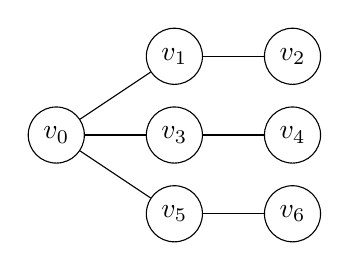
\begin{tikzpicture}[every node/.style={circle, draw}]
    \node (v0) at (0,0) {$v_0$};
    \node (v1) at (1.5,1) {$v_1$};
    \node (v2) at (3,1) {$v_2$};
    \node (v3) at (1.5,0) {$v_3$};
    \node (v4) at (3,0) {$v_4$};
    \node (v5) at (1.5,-1) {$v_5$};
    \node (v6) at (3,-1) {$v_6$};

    \draw (v0) -- (v1);
    \draw (v1) -- (v2);
    \draw (v0) -- (v3);
    \draw (v3) -- (v4);
    \draw (v0) -- (v5);
    \draw (v5) -- (v6);
\end{tikzpicture}
    \end{figure}

The greedy algorithm would yield the set $ \left\{ v_0, v_2, v_4, v_6\right\}$ as a solution. This, however, is not the optimal solution, which would be $U = \left \{ v_1, v_3, v_5\right \}$.

    \item The maximum degree of any vertex in $L$ must be $n-1$. For each $2 \leq i \leq n$, vertices in $R_i$ will connect to distinct vertices in $L$.  This means that at most $n-1$ connections will be made to the vertices in $R$ because we have $n - 1$ distinct degrees from the given range of $i$ values.\\

Running the greedy heuristic aglorithm will then first pick the vertex in $R$ with degree $n$ as we know there must be one. Each time we remove the incident edges to the vertex, we are reducing the maximum degree of the vertices in $L$, meaning we will continue to pick the vertices in $R$. It's clear that $|R| > n$, however, the optimal case should be just choosing the elements in $L$, with $|L| = n$.

    \item As discussed in the previous part, we must have $\lvert \compproblem{GreedyVertex} \rvert = |R|$. So, we have

\begin{align*}
	|R| &= \sum_{i=2}^n \left \lfloor \dfrac{n}{i} \right \rfloor\\
	&> \sum_{i=2}^n \left( \dfrac{n}{i} - 1\right)\\
	&= n\sum_{i=2}^n\left( \dfrac{1}{i} \right) - (n-1)\\
	&= n(H_n - 1) - (n-1)\\
	&= n(H_n - 2) + 1.
\end{align*}

Since $|R| > n(H_2 -2) + 1$, it must be so that $|R| \geq n(H_n - 2)$, which completes the proof.
    
    \item We know that the optimal solution is $|L| - n$, so 

\begin{align*}
	\frac{\lvert \compproblem{GreedyVertex} \rvert}{\lvert \compproblem{opt} \rvert}  &\geq \dfrac{n(H_n - 2)}{n}\\
&= H_n - 2.
\end{align*}

As $n$ grows, the error increases at a rate of $O(H_n) = O(\log n)$, which implies that the algorithm can perform arbitrarily badly.
\end{enumerate}
\end{solution}
\end{document}